\documentclass[conference]{IEEEtran}
\IEEEoverridecommandlockouts
\usepackage{cite}
\usepackage{amsmath,amssymb,amsfonts}
\usepackage{algorithmic}
\usepackage{graphicx}
\usepackage{textcomp}
\usepackage{xcolor}
\usepackage{subfig}
\usepackage{siunitx}
\usepackage{cleveref}
\usepackage{tikz}

\def\BibTeX{{\rm B\kern-.05em{\sc i\kern-.025em b}\kern-.08em
    T\kern-.1667em\lower.7ex\hbox{E}\kern-.125emX}}

\usepackage{eso-pic}
\newcommand\AtPageUpperCenter[1]{\AtPageUpperLeft{%
 \put(\LenToUnit{\dimexpr0.5\paperwidth-0.5\textwidth\relax},\LenToUnit{-1cm}){%
     \parbox{\textwidth}{\centering\fontsize{9}{11}\selectfont #1}}%
}}

\newcommand{\conf}[1]{%
\AddToShipoutPictureBG*{%
\AtPageUpperCenter{#1}%
}%
}

\conf{25th International Symposium INFOTEH-JAHORINA, 18-20 March 2026}

\begin{document}

\title{Combined Hall-Sensor Calibration and MTPA Control for BLDC Motors with Large Stator Inductance}

\author{\IEEEauthorblockN{Ryan Edric Nashota}
\IEEEauthorblockA{\textit{Mechanical Engineering} \\
\textit{University of British Columbia}\\
Vancouver, Canada \\
rnashota@student.ubc.ca}
\and
\IEEEauthorblockN{Mark Phung}
\IEEEauthorblockA{\textit{Engineering Physics} \\
\textit{University of British Columbia}\\
Vancouver, Canada \\
marklong@student.ubc.ca}
\and
\IEEEauthorblockN{Juri Jatskevitch}
\IEEEauthorblockA{\textit{Electrical and Computer Engineering} \\
\textit{University of British Columbia}\\
Vancouver, Canada \\
jurij@ece.ubc.ca }}

\maketitle

\begin{abstract}
Brushless DC (BLDC) motors are extensively utilized in industrial applications, yet they frequently encounter performance limitations due to Hall-sensor misalignment and significant stator inductance. These non-idealities manifest as torque ripple, acoustic noise, and a reduction in torque-per-ampere capability. This paper presents a unified control strategy that synergizes a lookup-table (LUT) based Hall-sensor calibration with a Maximum Torque Per Ampere (MTPA) Proportional-Integral (PI) controller. The proposed calibration routine employs an extrapolated averaging technique to rectify commutation intervals without introducing filter delays. Concurrently, the MTPA controller dynamically compensates for the current phase lag by adjusting the advance firing angle, thereby driving the average d-axis current to zero. Verification through detailed machine simulations confirms that the combined approach effectively restores balanced commutation and enhances torque generation efficiency compared to uncompensated baselines.
\end{abstract}

\begin{IEEEkeywords}
BLDC motor, Hall-sensor misalignment, MTPA, Lookup Table (LUT), Advance Angle Control.
\end{IEEEkeywords}

\section{Introduction}
\label{sec:introduction}
\subsection{Background}
Brushless DC (BLDC) motors are widely used in modern industries such as electric mobility, 
robotics, manufacturing, and industrial automation due to their high power density, good 
reliability and efficiency, superior torque-speed characteristics, simplicity, and low cost 
\cite{b3, b4}. Among various motor drive methods, Hall-sensor-controlled BLDC machines 
are commonly chosen for their ability to operate at a wide range of speeds and in applications 
where sensorless control may not be preferred \cite{b3, b4}.

A BLDC motor consists of a permanent magnet synchronous machine (PMSM), which is electronically 
commutated by a voltage source inverter (VSI). A schematic diagram of a typical BLDC motor drive 
is shown in Fig. 1-1, where the VSI is controlled using three Hall sensors that detect the rotor 
position \cite{b5}. Each Hall sensor outputs a square wave signal with a value of 1 or 0, 
depending on the rotor position. To provide six evenly spaced readings, the three Hall sensors 
must be spaced apart by 120$^\circ$ \cite{b5}. In the 120$^\circ$ commutation scheme used in 
this work, each phase conducts for two-thirds of the electrical cycle \cite{b7}. In common 
operating mode (COM), the VSI shifts its switching by 30$^\circ$ ahead of the Hall state 
transitions \cite{b8}. When stator inductance is negligible, this control mode aligns the 
fundamental component of the phase current with the phase back electromotive force (EMF), thus 
enabling maximum torque-per-ampere (MTPA) operation \cite{b8}. However, motors with significant 
stator inductance require dynamic adjustment of the advance firing angle to maintain MTPA 
operation.

\begin{figure}[htbp]
\centerline{\includegraphics[width=0.8\columnwidth]{figures/1.vsi_background.jpg}}
\caption{Diagram for a Hall-sensor controlled BLDC motor driven by a VSI. The misaligned Hall sensors are passed through the proposed 
algorithm.}
\label{fig:vsi_background}
\end{figure}
Manufacturing imperfections cause the Hall sensors to deviate from their intended 120$^\circ$ 
spacing, resulting in asymmetric commutation timing as shown in \Cref{fig:hall_sensor_comparison}. This leads to imbalanced currents across phases, elevated 
torque oscillations, and overall degradation of motor performance \cite{b6, b7, b8, b9}. Signal 
conditioning techniques, including moving average filters, have been applied to Hall sensor 
outputs \cite{b9, b10}, yet these introduce timing delays that further compromise MTPA alignment. 
In motors with large winding inductance, proportional-integral controllers have been developed to 
dynamically adjust the commutation advance angle \cite{b7, b11, b12}. However, these compensation 
strategies rely on accurate rotor position estimation, which becomes unreliable when the Hall 
sensors themselves are misaligned.


This paper builds upon previous work and presents a practical dual-strategy approach combining lookup table (LUT) calibration \cite{b2} 
with dynamic MTPA advance angle control \cite{b1} to simultaneously correct for Hall sensor positioning errors and 
compensate for inductance-related phase lag in 120$^\circ$ commutation mode. The proposed method 
is validated through simulation using MATLAB/Simulink on an industrial BLDC motor model 
exhibiting significant Hall misalignment and high winding time constant.


\section{Modeling of the BLDC Motor Drive System}
\label{sec:modeling}
The modeling of the BLDC motor is based on typical system as referenced in \Cref{fig:vsi_background}. 
\subsection{Mathematical Model of the PMSM}
The BLDC motor is modeled as a surface-mounted Permanent Magnet Synchronous Machine (PMSM). The stator voltage equation in the stationary reference frame is expressed as:
\begin{equation}
    \mathbf{v}_{abc} = R_s \mathbf{i}_{abc} + L_s \frac{d}{dt}\mathbf{i}_{abc} + \mathbf{e}_{abc}
    \label{eq:voltage}
\end{equation}
where $\mathbf{v}_{abc}$, $\mathbf{i}_{abc}$, and $\mathbf{e}_{abc}$ are the phase voltage, current, and back-EMF vectors respectively. $R_s$ is the stator resistance and $L_s$ is the synchronous inductance.

The electromagnetic torque $T_e$ is given by the interaction of the phase currents and back-EMF:
\begin{equation}
    T_e = \frac{1}{\omega_m} \sum_{k \in \{a,b,c\}} e_k i_k
    \label{eq:torque_general}
\end{equation}
where $\omega_m$ is the mechanical angular velocity.

To implement the MTPA control, it is convenient to transform the system variables into the synchronous rotating $dq$ reference 
frame using the Park transformation matrix $\mathbf{K}_s^r(\theta_r)$:
\begin{equation}
    \mathbf{K}_s^r(\theta_r) = \frac{2}{3} \begin{bmatrix}
    \cos(\theta_r) & \cos(\theta_r - \frac{2\pi}{3}) & \cos(\theta_r + \frac{2\pi}{3}) \\
    \sin(\theta_r) & \sin(\theta_r - \frac{2\pi}{3}) & \sin(\theta_r + \frac{2\pi}{3}) \\
    1/2 & 1/2 & 1/2
    \end{bmatrix}
    \label{eq:park}
\end{equation}

Applying this transformation to \eqref{eq:voltage} yields the dynamic equations in the $dq$ frame:
 \begin{align}
     v_q &= R_s i_q + L_s \frac{di_q}{dt} + \omega_r L_s i_d + \omega_r \psi_m \label{eq:vq} \\
     v_d &= R_s i_d + L_s \frac{di_d}{dt} - \omega_r L_s i_q \label{eq:vd}
 \end{align}
 where $\omega_r = P\omega_m$ is the electrical rotor speed and $\psi_m$ is the permanent magnet flux linkage. The electromagnetic torque is given by:
 \begin{equation}
     T_e = \frac{3P}{2} \left[ \psi_m i_q + (L_d - L_q) i_d i_q \right]
     \label{eq:torque}
 \end{equation}
 For a surface-mounted PMSM ($L_d = L_q = L_s$), the reluctance torque term vanishes. 
 Hence, notice that in \eqref{eq:torque}, the $d$-axis current $i_d$ does not contribute 
 to the output torque and thus creates more losses per ampere. Ideally, to maximize torque efficiency, 
 we should design a controller that aims to maintain $i_d = 0$. In the context of six-step operation, this translates to 
 keeping the time average of the $d$-axis current magnitude close to zero \cite{b1, b7}. 

 \subsection{Limitations of Conventional Six-Step Commutation}
 In standard 120$^\circ$ commutation, the ideal switching instants are synchronized with the rotor position to maximize torque. 
 Geometrically, this corresponds to keeping the stator flux vector perpendicular to the rotor flux. Ideally, this requires the commutation 
 to occur 30$^\circ$ electrical after a Hall state transition (assuming zero alignment offset), effectively centering the 60$^\circ$ conduction block around 
 the peak back-EMF. However, this static 30$^\circ$ shift (Common Operating Mode) is only valid when the stator current reacts instantly to voltage changes.
 
 In practice, the stator winding inductance ($L_s$) introduces a time delay in the current rise, 
 governed by the dynamic voltage equations \eqref{eq:vq} and \eqref{eq:vd}. As rotor speed increases, 
 the inductive reactance term $\omega_r L_s$ becomes significant, causing the phase current to lag 
 behind the back-EMF. This misalignment reduces the effective torque-producing current component $i_q$ 
 in \eqref{eq:torque}, while simultaneously increasing the non-torque-producing $d$-axis component $i_d$, 
 representing increased losses. To recover MTPA performance, the commutation angle must be advanced by an additional angle $\phi_{adv}$ to 
 compensate for this inductive lag, ensuring the current waveform remains in phase with the back-EMF.

 \subsection{Effects of Hall Sensor Position Error}
 As a result of manufacturing tolerances, Hall sensors in motors typically deviate from their 
 ideal 120$^\circ$ spacing. As visualized in \Cref{fig:hall_sensor_misaligned_physical}, these 
 angular offsets distort the duration of the conduction intervals, causing some phases to conduct 
 for longer or shorter than the intended 60 electrical degrees. This asymmetry introduces 
 significant low-frequency torque oscillations.

 \begin{figure}[htbp]
 \centerline{\includegraphics[width=0.6\columnwidth]{figures/hall_sensor_misaligned_physical.png}}
 \caption{Manufacturing tolerances in Hall sensor placement leads to misalignment from ideal 120$^\circ$ spacing.}
 \label{fig:hall_sensor_misaligned_physical}
 \end{figure}
 
 The uneven switching intervals due to Hall sensor misalignment degrades the performance of any dynamic 
 advance angle controller such as MTPA. The MTPA strategy relies on calculating the average $d$-axis current 
 ($\bar{i}_d$) over a sector. If the sector duration itself is corrupted by Hall misalignment, 
 the calculated $\bar{i}_d$ becomes inaccurate, leading to incorrect firing angle 
 adjustments and potential instability.
 
 Prior research has utilized moving average filters to smooth these intervals \cite{b1}. 
 The filters, while effective in steady-state, introduce a measurement delay, 
 causing the estimated speed to lag the actual speed during transients. 
 This delay prevents the MTPA controller from reacting quickly to load or speed changes. 
 To address this, a Lookup Table (LUT) based calibration method \cite{b2} is employed in this work. 
 By identifying the errors offline and applying a pre-computed correction, the LUT 
 approach eliminates runtime delays, which improves transient performance. The advantage of no delay
 also suggests an accurate speed estimation, which is critical for practical motor control applications.

 \begin{figure}[htbp]
 \centerline{\includegraphics[width=\columnwidth]{figures/hall_sensor_comparison_paper.png}}
 \caption{Visualization of Hall sensor misalignment on the stator and the resulting distortion in switching intervals.}
 \label{fig:hall_sensor_comparison}
 \end{figure}

\section{Hall Sensor Signals Filter via Extrapolated Averaging}
\label{sec:hall_filter}
To correct the commutation asymmetry while preserving dynamic performance, we first examine conventional filtering approaches and then propose a Lookup Table (LUT) based strategy that eliminates their inherent delays.

\subsection{Evaluation of Existing Averaging Filters}
Packet-based averaging filters are often employed to smooth the irregular Hall intervals. Several such extrapolating filters have been proposed, including 3-step and 6-step variants \cite{b9}. The correction terms for the 3-step ($\tau_{a3}^{corr}$) and 6-step ($\tau_{a6}^{corr}$) averaging filters are given by:
\begin{equation}
    \tau_{a3}^{corr}(n) = \frac{1}{3}(\tau(n-2) + 2\tau(n-3))
    \label{eq:tau_a3}
\end{equation}
\begin{equation}
    \tau_{a6}^{corr}(n) = \frac{1}{3}(-\tau(n-1) + \sum_{k=3}^{6}\tau(n-k))
    \label{eq:tau_a6}
\end{equation}
These filters have been shown to balance the Hall-sensor errors successfully in steady state, ensuring even conduction intervals. However, the critical drawback is that any such averaging filter inherently possesses memory. This results in a computational delay and compromises the transient performance of the drive, as the filter output lags behind the actual speed changes. This lag is particularly detrimental for the MTPA loop which requires accurate instantaneous position and speed feedback.

\subsection{Proposed LUT-Based Calibration Strategy}
To overcome the bandwidth limitation of runtime filters, this work utilizes an offline calibration approach. The misalignment characteristics are identified during a dedicated initialization phase and stored, allowing for zero-delay correction during operation.

During the calibration mode, the motor is driven to a steady reference speed. A Recursive Least Squares (RLS) style moving average filter is temporarily engaged to stabilize the measured Hall intervals against jitter. Let $\tau(n)$ be the measured interval:
\begin{equation}
    \bar{\tau}(n) = \alpha \tau(n) + (1-\alpha) \bar{\tau}(n-1)
    \label{eq:moving_avg}
\end{equation}
where $\alpha$ is a forgetting factor. Once the speed is stable, the ideal sector duration $\tau_{ideal}$ is computed as the average over a full mechanical rotation ($N=6$ for one pole pair):
\begin{equation}
    \tau_{ideal} = \frac{1}{N} \sum_{k=1}^{N} \tau(n-k)
    \label{eq:tau_ideal}
\end{equation}
For each Hall state $S$, the specific time error $\delta_t[S]$ is identified as the deviation from this ideal average:
\begin{equation}
    \delta_t[S] = \tau_{meas}[S] - \tau_{ideal}
    \label{eq:time_error}
\end{equation}
This time error is converted into an angular correction value $\Delta \theta_{LUT}[S]$ using the estimated electrical speed $\hat{\omega}_e$, and stored in a non-volatile Lookup Table (LUT):
\begin{equation}
    \Delta \theta_{LUT}[S] = \hat{\omega}_e \cdot \delta_t[S]
    \label{eq:lut_angle}
\end{equation}

\subsection{Runtime Correction}
During normal runtime operation, the averaging filters are bypassed. Instead, the controller retrieves the stored correction angle $\Delta \theta_{LUT}$ corresponding to the impending sector. The corrected commutation time interval $\tau_{LUT}^{corr}$ is predicted as:
\begin{equation}
    \tau_{LUT}^{corr}(n) = \frac{\pi/3 - \Delta \theta_{LUT}[S]}{\hat{\omega}_e}
    \label{eq:tau_lut}
\end{equation}
The commutation instant $t_{out}$ is then scheduled:
\begin{equation}
    t_{out}(n) = t_{in}(n) + \tau_{LUT}^{corr}(n)
    \label{eq:t_out}
\end{equation}
This feed-forward mechanism cancels the geometric misalignment error without introducing the phase lag associated with real-time averaging, thus preserving the system's dynamic response capability.

\section{MTPA PI Controller via Advance Angle Compensation}
\label{sec:mtpa_control}
With the Hall signal timing balanced, the control system leverages an MTPA loop to optimize torque production.

\subsection{Control Strategy}
For a surface-mounted PMSM, maximum torque per ampere is achieved when the stator current vector is orthogonal to the rotor flux, implying $i_d = 0$. However, due to the prominent stator inductance term $\omega_r L_s i_d$ in \eqref{eq:vq}, a phase lag occurs at high speeds.

To counteract this, the controller computes the average $d$-axis current $\bar{i}_d$ over each conduction interval using the coordinate transformation defined in \eqref{eq:park}. An error signal $e_{id} = 0 - \bar{i}_d$ is processed by a PI controller to generate the optimal advance angle $\phi_v$:
\begin{equation}
    \phi_v[k] = K_p (0 - \bar{i}_d[k]) + K_i \sum_{j=0}^{k} (0 - \bar{i}_d[j]) \Delta t
    \label{eq:pi_ctrl}
\end{equation}
where $K_p$ and $K_i$ are the proportional and integral gains.

\begin{figure}[htbp]
\centering
\resizebox{\columnwidth}{!}{
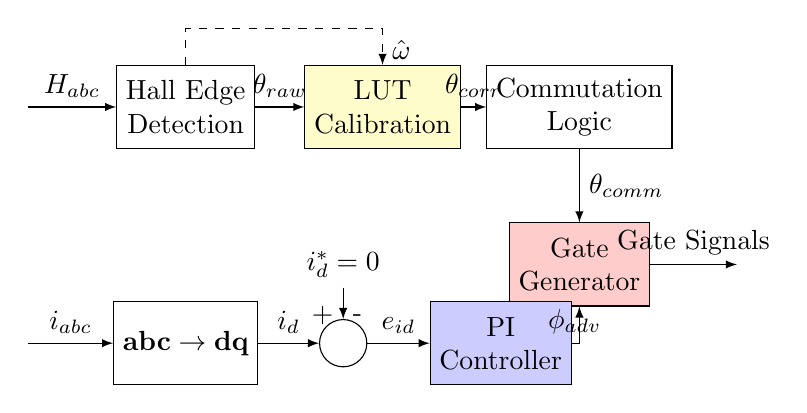
\begin{tikzpicture}[auto, node distance=1.5cm, >=latex,
    block/.style={draw, fill=white, rectangle, minimum height=3em, minimum width=3em, align=center},
    input/.style={coordinate},
    output/.style={coordinate},
    sum/.style={draw, fill=white, circle, inner sep=0pt, minimum size=6mm},
    pinstyle/.style={pin edge={to-,t,black,options={label={[font=\footnotesize]above:#1}}}}]

    % Nodes
    \node [input, name=input] {};
    \node [block, right of=input, node distance=2cm] (hall_proc) {Hall Edge\\Detection};
    \node [block, right of=hall_proc, node distance=2.5cm, fill=yellow!20] (lut) {LUT\\Calibration};
    \node [block, right of=lut, node distance=2.5cm] (comm_logic) {Commutation\\Logic};
    \node [block, below of=comm_logic, node distance=2cm, fill=red!20] (gate_gen) {Gate\\Generator};
    
    \node [block, below of=hall_proc, node distance=3cm] (clarke) {$\mathbf{abc} \to \mathbf{dq}$};
    \node [sum, right of=clarke, node distance=2cm] (sum) {};
    \node [block, right of=sum, node distance=2cm, fill=blue!20] (pi) {PI\\Controller};
    
    \node [output, right of=gate_gen, node distance=2cm] (output) {};

    % Arrows
    \draw [->] (input) -- node[name=halls] {$H_{abc}$} (hall_proc);
    \draw [->] (hall_proc) -- node {$\theta_{raw}$} (lut);
    \draw [->] (lut) -- node {$\theta_{corr}$} (comm_logic);
    \draw [->] (comm_logic) -- node[name=theta_comm] {$\theta_{comm}$} (gate_gen);
    
    % MTPA Loop
    \node [input, below of=input, node distance=3cm] (i_abc) {};
    \draw [->] (i_abc) -- node {$i_{abc}$} (clarke);
    \draw [->] (clarke) -- node {$i_d$} (sum);
    \node [above of=sum, node distance=1cm] (ref) {$i_d^*=0$};
    \draw [->] (ref) -- (sum) node[pos=0.9, right] {-} node[pos=0.9, left] {+};
    \draw [->] (sum) -- node {$e_{id}$} (pi);
    \draw [->] (pi) -| node[pos=0.2] {$\phi_{adv}$} (gate_gen);
    
    \draw [->] (gate_gen) -- node {Gate Signals} (output);
    
    % Speed feedback for LUT
    \draw [->, dashed] (hall_proc) -- ++(0,1) -| node[pos=0.8] {$\hat{\omega}$} (lut);

\end{tikzpicture}
}
\caption{Flowchart of the proposed combined control strategy. The Hall signals are calibrated via a LUT (Yellow) to provide accurate commutation timing. Simultaneously, the MTPA loop (Blue) adjusts the advance angle $\phi_{adv}$ to zero the d-axis current.}
\label{fig:control_flowchart}
\end{figure}

The total firing angle $\alpha$ applied to the VSI is the sum of the standard $30^\circ$ offset and the calculated advance:
\begin{equation}
    \alpha = 30^\circ + \phi_v
\end{equation}
This dynamic adjustment compensates for the inductive phase lag, ensuring the current vector remains aligned with the back-EMF ($q$-axis) across the operating speed range.

\section{Detailed Machine Simulations}
\label{sec:simulation}
The proposed combined control strategy was validated using a high-fidelity BLDC motor model.

\subsection{Steady-State Performance}
The effectiveness of the method is demonstrated by observing the alignment of phase currents and back-EMF. \Cref{fig:alignment} compares the uncompensated case (a), the filter-only case (b), and the combined Method (c). The uncompensated waveforms show significant distortion and phase lag. The filter balances the switching intervals, but the phase lag persists. The combined method (c) achieves both balanced intervals and optimal phase alignment.

\begin{figure}[htbp]
\centerline{\includegraphics[width=\columnwidth]{C:/Users/gyang/.gemini/antigravity/brain/b08294ba-f3f3-4f5f-9c56-ce80970f78f6/uploaded_image_3_1765166842486.png}}
\caption{Alignment of the fundamental phase current and back-EMF: (a) uncompensated; (b) filter only; (c) combined filter + MTPA controller.}
\label{fig:alignment}
\end{figure}

\Cref{fig:results_torque} presents the steady-state performance comparison in terms of torque generation efficiency, defined as the ratio of average torque to RMS phase current ($K_t = \bar{T}_e / I_{rms}$). The uncompensated case exhibits the lowest efficiency due to significant phase misalignment. The filter-only approach improves commutation symmetry but introduces delays that prevent optimal torque production. The proposed combined method (LUT + MTPA) demonstrates the highest torque-per-ampere ratio, confirming that the algorithm successfully compensates for both Hall sensor placement errors and inductive phase lag, thereby recovering the optimal operating point.

\begin{figure}[htbp]
\centerline{\includegraphics[width=\columnwidth]{figures/torque_comparison_paper.png}}
\caption{Comparison of Torque Generation Efficiency (Torque Constant $K_t$) across four operating cases. The proposed LUT + MTPA method achieves the highest torque-per-ampere, indicating optimal alignment.}
\label{fig:results_torque}
\end{figure}

\subsection{Transient Performance}
To verify the robustness of the proposed control, transient response tests were conducted.

\Cref{fig:transient_compare} shows a comparison of the current response during startup. The uncompensated case shows large current spikes, while the proposed method smooths the current envelope. \Cref{fig:transient_stacked} provides a detailed view of the phase currents with and without compensation.

\begin{figure}[htbp]
\centerline{\includegraphics[width=\columnwidth]{figures/current_transient_compare.png}}
\caption{Comparison of phase current transients during startup. The proposed method (Red) reduces peak overshoot compared to uncompensated (Blue).}
\label{fig:transient_compare}
\end{figure}

\begin{figure}[htbp]
\centerline{\includegraphics[width=\columnwidth]{figures/current_transient_stacked_inset.png}}
\caption{Stacked view of phase currents, highlighting the zoomed-in improvement in waveform quality.}
\label{fig:transient_stacked}
\end{figure}

\Cref{fig:speed_step} illustrates the speed response of the motor to a step command. The yellow trace representing the proposed LUT correction demonstrates a response time comparable to the ideal sensor placement (blue trace), significantly outperforming the 3-step and 6-step averaging filters which introduce noticeable delays and overshoot.

\begin{figure}[htbp]
\centerline{\includegraphics[width=\columnwidth]{figures/speed_step_placeholder.png}}
\caption{Simulated speed response step increase. (a) with ideal Hall sensor placement; (b) Comparison of averaging filters vs. proposed LUT correction. The LUT method achieves faster convergence.}
\label{fig:speed_step}
\end{figure}

\Cref{fig:load_step} depicts the system response to a sudden load torque step. The LUT-based controller maintains stability and exhibits superior torque dynamic performance. The speed dip is minimized, and the electromagnetic torque recovers smoothly without the oscillatory behavior observed in the conventional averaging methods.

\begin{figure}[htbp]
\centerline{\includegraphics[width=\columnwidth]{figures/torque_step_placeholder.png}}
\caption{Simulated response to a load step increase: (a) speed response; (b) electromagnetic torque response. The proposed LUT correction (yellow trace) shows superior dynamic tracking.}
\label{fig:load_step}
\end{figure}

\section{Conclusion}
\label{sec:conclusion}
This paper presented a unified control framework addressing two critical performance bottlenecks in BLDC drives: sensor misalignment and inductive lag. By integrating a LUT-based calibration with a dynamic MTPA controller, the system achieves smooth and efficient operation. Simulation results confirm the method's ability to minimize torque ripple and maximize torque-per-ampere, while maintaining excellent transient response characteristics suitable for dynamic industrial applications.

\appendix[Motor Parameters]
The main parameters of the BLDC motor used in this study are listed in Table \ref{tab:motor_params}.
\begin{table}[htbp]
\caption{Motor Parameters}
\begin{center}
\begin{tabular}{|c|c|c|}
\hline
\textbf{Parameter} & \textbf{Symbol} & \textbf{Value} \\
\hline
Stator Resistance & $R_s$ & \SI{0.5}{\ohm} \\
\hline
Stator Inductance & $L_s$ & \SI{1.2}{mH} \\
\hline
Flux Linkage & $\psi_m$ & \SI{0.05}{Wb} \\
\hline
Pole Pairs & $P$ & 4 \\
\hline
Rated Speed & $\omega_{rated}$ & \SI{3000}{rpm} \\
\hline
\end{tabular}
\label{tab:motor_params}
\end{center}
\end{table}

\section*{Acknowledgment}
The authors acknowledge the support of the Department of Electrical and Computer Engineering at the University of British Columbia.

\begin{thebibliography}{00}
\bibitem{b1} M. Phung, ``Maximum Torque per Ampere Control of Brushless DC Motors with Large Winding Time Constant and Hall-Sensor Misalignment,'' BASc Thesis, University of British Columbia, Vancouver, BC, 2025.
\bibitem{b2} M. Hasman, ``Mitigating Misaligned Hall Sensors in BLDC Motors Using a Calibration Routine for Improved Fast Electromechanical Transients,'' BASc Thesis, University of British Columbia, Vancouver, BC, 2025.
\bibitem{b3} P. C. Krause, O. Wasynczuk, and S. D. Sudhoff, \emph{Analysis of Electric Machinery and Drive Systems}, 2nd ed., Piscataway, NJ: IEEE Press, 2002.
\bibitem{b4} P. Pillay and R. Krishnan, ``Modeling, simulation, and analysis of permanent-magnet motor drives, part II: The brushless DC motor drive,'' \emph{IEEE Trans. Ind. Appl.}, vol. 25, no. 2, pp. 274--279, Mar./Apr. 1989.
\bibitem{b5_book} P. C. Krause, O. Wasynczuk, S. Pekarek, and T. O'Connell, \emph{Electromechanical Motion Devices: Rotating Magnetic field-based Analysis with Online Animations}. Hoboken, NJ: Wiley-IEEE Press, 2020.
\bibitem{b5} D.-K. Kim, K.-W. Lee, and B.-I. Kwon, ``Commutation torque ripple reduction in a position sensorless brushless DC motor drive,'' \emph{IEEE Trans. Power Electron.}, vol. 21, no. 6, pp. 1762--1768, Nov. 2006.
\bibitem{b6} Y. Liu, Z. Q. Zhu, and D. Howe, ``Commutation-torque-ripple minimization in direct-torque-controlled PM brushless DC drives,'' \emph{IEEE Trans. Ind. Appl.}, vol. 43, no. 4, pp. 1012--1021, Jul./Aug. 2007.
\bibitem{b7} R. C. Osgood, ``Hall Effect Sensor Misalignment Correction in BLDC Motors,'' \emph{IEEE Trans. Ind. Electron.}, vol. 58, no. 9, 2011.
\bibitem{b8} J. Fang, ``Torque ripple minimization in BLDC motors with vector control,'' \emph{IEEE Trans. Magn.}, vol. 45, no. 1, 2009.
\bibitem{b9} S. Song, ``Averaging filter for Hall sensor error correction,'' \emph{IEEE Trans. Power Electron.}, vol. 28, 2013.
\bibitem{b10} H. Wang, ``Digital filter design for BLDC drives,'' \emph{Conf. Rec. IEEE IAS}, 2015.
\bibitem{b11} K. I. Hwu, ``Phase Advance Control for BLDC,'' \emph{IEEE Trans. Power Electron.}, 2010.
\bibitem{b12} C. Xia, ``Automatic Phase Advance,'' \emph{IEEE Trans. Energy Convers.}, 2016.
\end{thebibliography}

\end{document}
